\documentclass[10pt,twocolumn,letterpaper]{article}

\usepackage{iccv}
\usepackage{times}
\usepackage{epsfig}
\usepackage{graphicx}
\usepackage{amsmath}
\usepackage{amssymb}
\usepackage[caption=false]{subfig}

\usepackage[pagebackref=true,breaklinks=true,letterpaper=true,colorlinks,bookmarks=false]{hyperref}

\iccvfinalcopy

\def\iccvPaperID{****} % *** Enter the ICCV Paper ID here
\def\httilde{\mbox{\tt\raisebox{-.5ex}{\symbol{126}}}}

% Pages are numbered in submission mode, and unnumbered in camera-ready
\ificcvfinal\pagestyle{empty}\fi
\begin{document}

%%%%%%%%% TITLE
\title{3D Photography - Final Report}

\author{Jan Rueegg\\
ETH Zurich\\
{\tt\small rggjan@gmail.com}
% For a paper whose authors are all at the same institution,
% omit the following lines up until the closing ``}''.
% Additional authors and addresses can be added with ``\and'',
% just like the second author.
% To save space, use either the email address or home page, not both
\and
Remo Meyer\\
ETH Zurich\\
{\tt\small meyerre@student.ethz.ch}
}

\maketitle
\thispagestyle{empty}

%%%%%%%%% ABSTRACT
\begin{abstract}
Some general explanation, maybe copy from proposal %TODO
\end{abstract}

\section{Classical ICP Algorithm}
The core of our implementation is the alignement of 2 pointclouds. 
We have devided this functionality into 4 subfunctions (Selection, Matching, Rejection and Minimization), described below. This is very
similar to the steps described in the Fast ICP paper (\cite{fasticp}). As described there, we didn't use any weighting of the points,
because it is considered nt to bring any advantage according to the paper.

\subsection{Selection}
First we have to choose which points we want to align. This process is called selection. 
We have choosen to sample the points randomly. 
This has several advantages as it is fast, easy to implement and each point has potentially an influence on the algortihm, what is good.

Also, we only sample points in one image, and then match them to the points in the second image. This has several reasons, one of them
being able to match against a global point cloud, without having to estimate the normals and projection matrix in both clouds.
This is explained in more detail below.

\subsection{Matching}
\label{backprojection}

Initially we matched each selected point with it's nearest point in the target cloud. 
This generally works, but has several downsides: First it was slow, especially without an accelerated search structure (e.g. kd-tree). 
Furthermore, this seems to be less stable than other matching approaches, according to the Fast ICP paper (\cite{fasticp}).

So we went for a projection based approach: We first take the selected point and translate it into the coordinate system of the other camera,
using our current best guess of the translation / rotation we calculated so far. In a second step, we simply backproject it with the second camera,
and receive basically the x and y coordinates of the pixels containing the matched points in the other image. If these coordinates are outside the image,
we can simply discard the original point and select a new one.

This is very fast as each point can be matched in O(1) (assuming not too many of the projected points lie outside of the image), opposite to
O(\# selected points) using the old method.

We later extended this approach with a search for compatible points: We look into the neighbourhood of the backprojected point
for the point with the best matching color information (measuring euclidian distance in RGB space). See section \ref{colormatching}.

\subsection{Rejection}
To avoid too strong influence of outliers respectively wrong matches, we reject points that are to far away of each other. 
To decide which matches are too far away, we computed the average distance. Then we multiply this average with some constant
factor (\textit{1.2}, in our case), and use this value as a threshold: All the matches that have a distance greater than this
we can now discard.

\subsection{Minimization}
\label{minimization}
Now having all the matched points and their normals, we have to find a transformation matrix which minimizes the distance between those matched points.
As the camera is always the same and does not change it can only have made a translation or a rotation, resulting in a matrix with 6 degrees of freedom.

As a minimization criterium we used a point-to-plane metric: We try to minimize, in a least squares sense, the distance of each point to the plane
defined by the other point and its normal. Although this gives us a nonlinear equation system, it can be easily linearized under the assumption
that the angles of the rotation are really small. As described in \cite{ptp}, this problem can then be solved quite efficiently using SVD.

In our code, we then solve this linear system with the eigen library (see section \ref{libraries}).
To compensate the error from linearizing the system, we first tried to run the minimization several times, what brings more accuracy for a single step. 
However as the solving of the system is one of the most time consuming tasks in this algorithm,
and most transformations have only a small part of rotation, it's better to make a new icp step than to make additional svd iterations.

\subsection{Optimizations}
We combined the Selection, matching and rejection step into one function. This allows us to have a constant number of samples,
which then gives us more freedom in setting the number of samples. In the beginning, it happened quite often that we had to discard
80\% or more of the chosen samples, this cannot happen anymore. Testing showed, that fewer samples(around 50) reduce the computation
time a lot, while keeping the accuracy at a reasonable level.

\section{Additional Steps}
Besides implementing the steps described in the ''Fast ICP''\cite{fasticp} paper,
we needed to implement some additional steps to get the algorithm working.

\subsection{Calibration}
To be able to do the backprojection described in Section \ref{backprojection}, we needed to have the projection matrix of the 3D-points
into the 2D camera pixel coordinates.
Although there was a projection matrix provided within the ROS environment, we were not sure how accurate this would be. Therefore, we
wrote all the points from multiple pictures out into a file, and calculated the projection matrix ourselves. 

For this, we used the Direct Linear Transform (DLT) algorithm written last Semester in the Computer Vision course.

\subsection{Normal estimation}
We decided to implement a point-to-plane error metric in the last step of the ICP Algorithm (section \ref{minimization}).
To use that, we needed to define a plane respectively a normal at each of the matched points.

Since the kinect framework does not provide any normal information, we had to generate them ourselves.
For that, we implemented and compared several different methods.

\subsubsection{Cross Product}
The first was to simply take the top/bottom/right/left neighbours and compute the normal with the crossproduct.
The advantage of this is that we can calculate the normal very fast, and only need a small neighbourhood around the point
we want the normal from.

However, the approach has some severe limitations, as if only one of the 4 neighbours is a \textit{NaN}
(due to the limitations in the kinect) the normal can't be computed.
Furthermore it is very sensitive to noise, and only one outlier can make the normal unusable.

\subsubsection{Principal Components}
So we aimed at a more stable solution which is based on the computation of the principal coponents: We gathered a number of neighbouring
points, starting from the point we want the normal from. From these, we generate the covariance Matrix and calculate the Eigenvectors.

Basically this is a principal component analysis: The first 2 principal components describe the tangential direction of
the plane while the 3th is the normal component.
Compared to the previous solution this is much slower, but much more stable and an arbitrary number of neighbouring points may be chosen.

\subsubsection{Extended Cross Product}
After it turned out that the Principac Componant analysis was quite slow, we decided to try a third method: What we did was basically take the Cross
Product again, but this time with four points that are a number of pixels \textbf{R} far away from the original pixel. So, instead of taking the closest
four points in any direction, we take for example the points 5 or 10 pixels away, when \textbf{R} is 5 or 10, respectively.

This has the effect that pixel noise has a much smaller influence on the result, but computation is still very fast. However, it has of course a much more
smoothing effect on the normals, and many small details can be lost.

\subsubsection{Comparison}
To be able to decide, how to make the trade-off between the number of computations and the accuracy, we made some visualizations of the computed
normals (see figure \ref{fig:normals}).

We varied the method and the size of the considered neighbourhood respectively the offset between the samples. You can clearly see that the simple cross
product (\ref{fig:crossproduct}) has the worst characteristics, especially on this noisy example. The data are from a wall that are very far away from
the kinect camera, giving only very coarse depth accuracy.

The principal components method (\ref{fig:variance}) and also the extended cross product (\ref{fig:extended}) show much better results. However, the
extended cross product method can only be used in areas where enough data points are availabe, meaning we have no normals at edges (the red dots in 
the figures) and in areas whith many \textit{NaN}'s. Also, PCA is much more robust and gives generally more stable result.

Therefore, in the end, we decided to still use PCA to calculate the normals in most cases. We found that a radius of 6 is a good compromise between
robustness on one side, and detail preserving and computational speed on the other side.

\begin{figure*}
  \centering
  \subfloat[Cross Product]{\label{fig:crossproduct}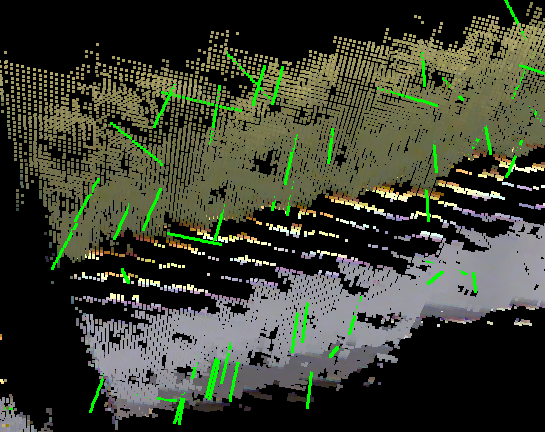
\includegraphics[width=0.3\textwidth]{simple1}}
  \quad
  \subfloat[Principal Components]{\label{fig:variance}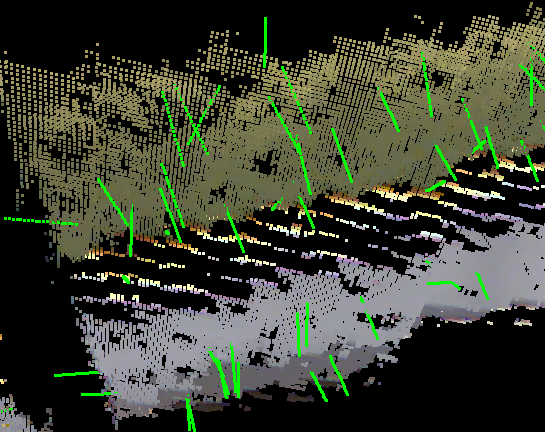
\includegraphics[width=0.3\textwidth]{variance8}}
  \quad
  \subfloat[Extended Cross Product]{\label{fig:extended}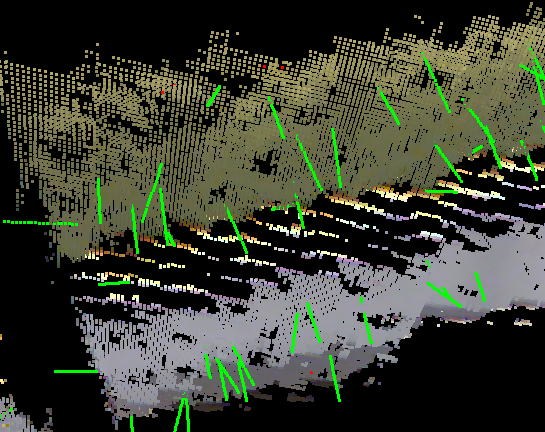
\includegraphics[width=0.3\textwidth]{simple8}}
  \caption{Different normal calculation methods}
  \label{fig:normals}
\end{figure*}

\subsection{Usage of Color}
\label{colormatching}
Compared to other Range scanners, with the kinect we have the possibility to also get the color information of the images.
This works not perfectly well, however: The resoulutions of the color camera and the infrared camera are different, and
they have also a certain offset, making it necessary to do some 3D-calculations to match them together.

Despite this, we tried to use the color information to get better results in the selection and matching step: After having
done the usual backprojection of the points from one range image into the other, we tried to look in a certain radius around
the projected point to find others with a more similar color in the 3D RGB - space. Especially on big planes or walls, with
no distinctive 3D features to use, color information could potentially give valuable information when there is some kind
of texture on the walls. But also for matching points from differently colored foreground and background objects color
information is useful.

For the radius, we did various experiments. The simplest was a fixed radius of up to 20 pixels. However, also other
possibilities were tried out, like having a big radius at the beginning, and making it smaller over time, to get a
better convergence, especially on surfaces without big color variances.

We found that the usage of color information can give a significant speedup, measured in the number of steps used for the
algorithm to converge. However, this was very dependend on the setting, and it could also lead to instability.
Furthermore it significantly increased computational time overall, what was not always made up with the reduced number of
steps. Thats why we didn't use color information in the demo at the end of the project.

We conclude here, that the color information could indeed be a big help matching corresponding points in the ICP algorithm,
however it would probably need a more elaborate matching (like patch comparisons or gradients) to get robust results.

\subsection{Hashing}
At the beginning, we always only matched two point clouds together. However, as soon as we have a countinious stream of images,
there are various new problems to be solved: On one hand, we needed a method to reduce the data: About 50 images (~ 2 Seconds)
gives us already 500 mb of data, what quickly fills the RAM if nothing is done about it. On the other hand, there is the problem
of global registration of all the images that needs to be solved. Simply comparing the last two images is not sufficiently accurate
to prevent a drift. We found that a simple hashing function solved many different problems related to multiple images.

\subsubsection{Compression}
To do a compression of the points, we first thought of building up a k-d tree over all the points of two images. In a next step, we could have
search for the two closest points in the pointcloud, and then merge them into one point. This could be iterated until sufficiently few
points remain in the tree. In this fashion, we could have this global tree over all the points already gathered, and continuously add new
images to that.

This would have been quite time consuming, however. Therefore, we thought of a similar, but much faster solution:
The general idea was to lay a 3D-grid over the image space, and then add at most one point into each Voxel. This means, that the resolution
of the grid determines how detailed the point cloud is. The advantage of this is that we can easily add the same (or a very similar) point cloud
to the structure without using more space.

Instead of using some structure like an octree to achieve this, we decided to use a hashtable to remember in which voxels we have already stored points:
Having a coordinate in x/y/z, we artificially decreased the accuracy of the coordinates to about cm or mm precision. Then we filled a big integer with
shifted versions of the points, and used this as starting hash value to place this in a set.

As an example: We have the Point
$$P = (1.123412\ldots, 2.188987\ldots, 3.889192\ldots)$$
First, we convert it to centimeters and round it to the integers $(112, 219, 389)$, then we add the three together:
$$\textit{hashvalue} = x + y*1000 + z*1000*1000 = 389 219 112$$

From this, we use a standard hash function and put in in the table. When we have a second
point that is very near this one, it gets mapped to the same hashvalue because of the rounding and we don't add it to the pointcloud.

\subsubsection{Global registration}
We also used this hashing to perform a global registration: Instead of always just matching two point clouds, as we did in the beginning, we started
to match the whole global point cloud with the new image. We hoped to achieve the following two things with this:
\begin{itemize}
\item Reduce drift. Because we always much against the whole history in a sense, we get less image-to-image drift over a whole sequence.
\item Have some kind of loop closure. Again, when we compare with the whole history, we can hope to be able to match against
the points of the first image, when we move the camera to the same place again.
\end{itemize}

This works because in the matching algorithm, we only need the projection matrix of
one of the point clouds, and also the normals of the points in one image. That means, when selecting the random points from the global point hash, it is
still possible to easily calculate the normals in one coherent kinect image, as well as doing the projection into this image.


\subsubsection{Accuracy calculation}
Using this hash function, we were also able to get a quite good measure for accuracy of matching between two images. We did the following:
\begin{enumerate}
\item Add all the points of the first point cloud to a hashset. This gives us the (low resolution) number of point in cloud 1 (\textit{= count1}).
\item Do the same for the second point cloud (\textit{= count2}).
\item Add all the points of both pointclouds to a hashset (\textit{= countsum}).
\item With this, the overlap between both pointclouds can easily calculated as \textit{(count1+count2-countsum)/(countsum)}.
\end{enumerate}
It turned out, that this overlap highly correlates with the matching accuracy: The better two clouds are matched, the more overlap they have, assuming
that only a small movement was performed, if the scene is general enough. For example, when you have two planes on top of each other, then the overlap
is 1. When one of them is a little bit moved in the direction of their normal, then the overlap drops quite fast to almost zero.

\subsubsection{Implementation}
We tried and profiled various implementations for the Hashset. The first two of them where the unordered set of the Boost library and the set of the
standard c library. However, both of them were too slow for our purposes, as (like described above) we have basically one insertion per pixel per image.

In a second step, we included the sparsehash library provided by google, which already gave us a speedup of about 2. Still, for 200 Iterations the
insertions took about 25 Seconds, what is way too slow.

Finally, we found that the \textit{bitset} datastructure of the standard c++ library was really fast, and for our resolution still memory efficient enough,
so we used that in our final implementation.

\section{Mesh generation}
As part of the \textit{GPGPU lecture}, we developed our project further and also generated a mesh out of the aligned pointclouds, as you can see in
Figure \ref{fig:pfostenmesh} for the merged \textit{pfosten} sequence (\ref{fig:pfostenend}).
As this is not part of this project, we will not go into detail about this, and just give a quick overview of what we did there.

\begin{figure}
  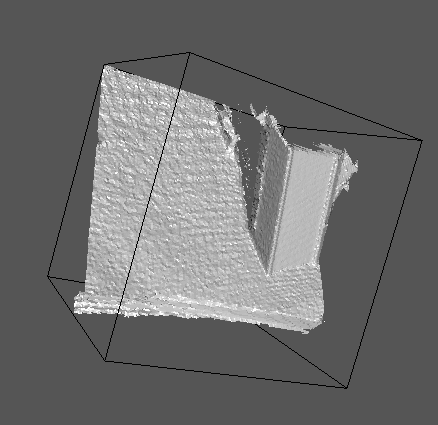
\includegraphics[width=0.4\textwidth]{pfostenmesh}
  \caption{Part of the generated mesh for the \textit{Pfosten} sequence}
  \label{fig:pfostenmesh}
\end{figure}

\section{Results}

\begin{figure}
  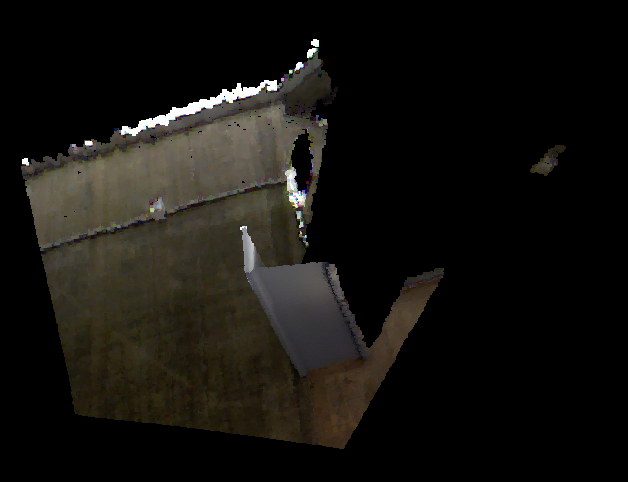
\includegraphics[width=0.5\textwidth]{pfostenstart}
  \label{fig:pfostenstart}
  \caption{First image of \textit{Pfosten} sequence}
\end{figure}

\begin{figure}
  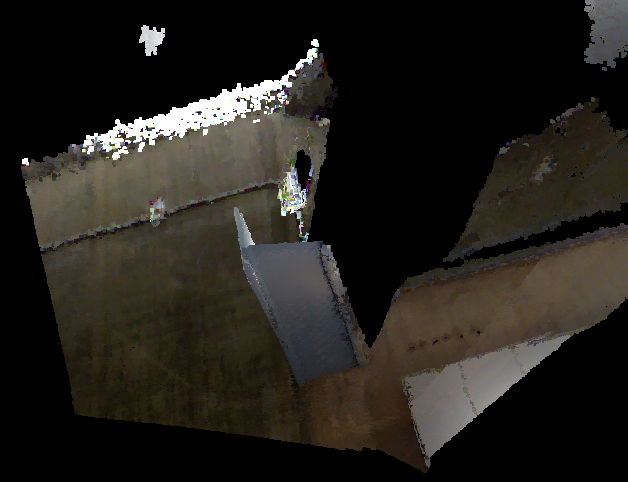
\includegraphics[width=0.5\textwidth]{pfostenend}
  \label{fig:pfostenend}
  \caption{Merged \textit{Pfosten} sequence}
\end{figure}

\begin{figure*}
  \centering
  \subfloat[First single image]{\label{fig:resultfirst}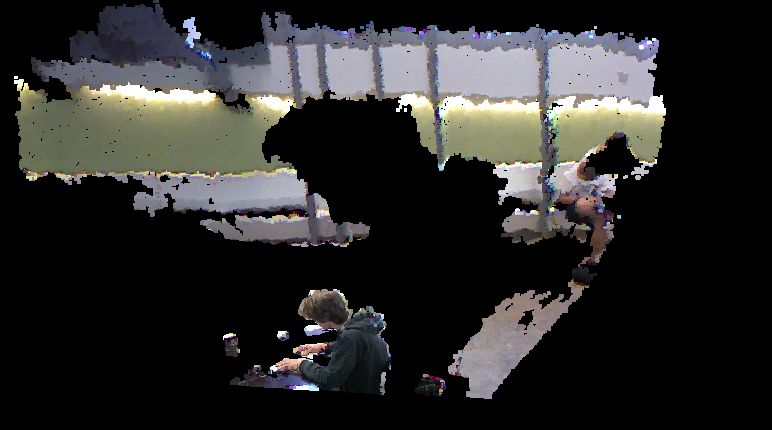
\includegraphics[width=0.33\textwidth]{resultfirst}}
  \subfloat[Merged cloud without hashing]{\label{fig:resultdrift}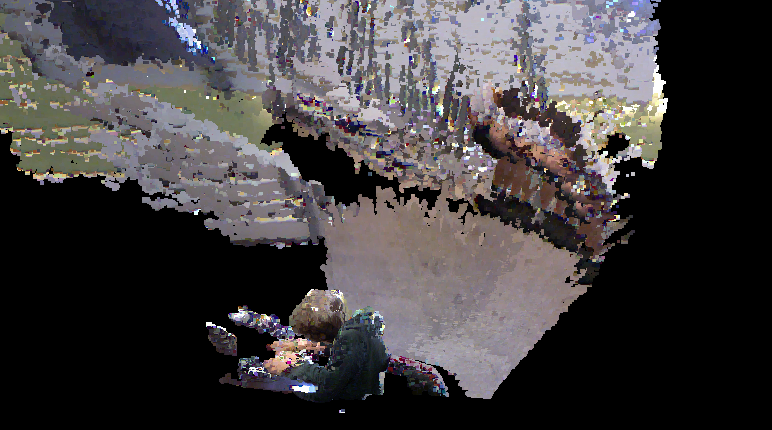
\includegraphics[width=0.33\textwidth]{resultdrift}}
  \subfloat[Merged cloud with hashing]{\label{fig:resulthashing}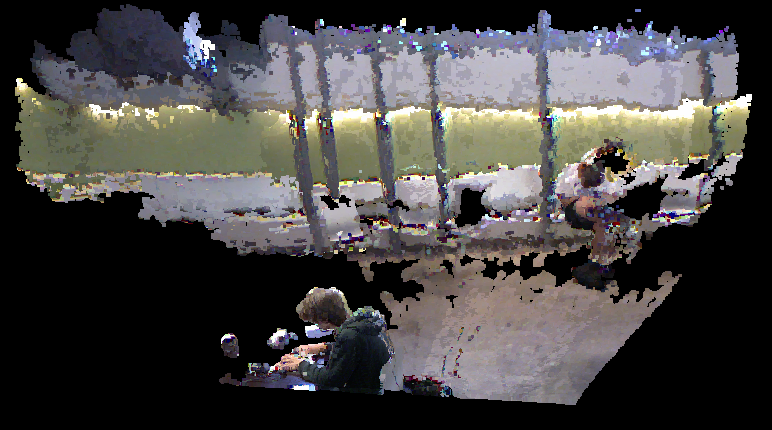
\includegraphics[width=0.33\textwidth]{resulthashing}}
  \caption{Merged \textit{ML} sequence with and without drift in global registration}
  \label{fig:globalregistration}
\end{figure*}


Realtime ... Hashing, new method (accuracy...) ... not too stable yet, more tuning/testing/different scenes needed ... extended cross product .. colors

\section{Discussion}

\section{Used libraries}
\label{libraries}
\begin{description}
\item[Eigen 2]
A lightweight C++ template library for vector and matrix math,
a.k.a. linear algebra.

\begin{itemize}
\item Point and matrix type declarations
\item SVD decomposition for normal computation and minimization
\end{itemize}

\href{http://eigen.tuxfamily.org}{http://eigen.tuxfamily.org}

\item[Robot Operating System (ROS)]
A meta-operating system for robots. It provides
language-independent and network-transparent communication for a
distributed robot control system.

\begin{itemize}
\item Register to kinect data
\item Send final point cloud and camera positions to mesh generation
\end{itemize}

\href{http://ros.org}{http//ros.org}

\item[Point Cloud Library (PCL)]
A comprehensive open source library for n-D Point Clouds and 3D geometry processing.

- - point cloud type definitions

\href{http://pointclouds.org}{http://pointclouds.org}

\item[The ROS OpenNI project]
ROS OpenNI is an open source project focused on the integration of the PrimeSense sensors with ROS.

-- kinect

\href{http://www.ros.org/wiki/ni}{http://www.ros.org/wiki/ni}

\end{description}

\begin{thebibliography}{99}
\bibitem{fasticp}
Szymon Rusinkiewicz and Marc Levoy.
\emph{Efficient Variants of the ICP Algorithm}.
Proceedings of the International Conference on 3-D Digital Imaging and
Modeling (3DIM), pp. 145–152, 2001.

\bibitem{ptp}
Kok-Lim Low.
\emph{Linear Least-Squares Optimization for
Point-to-Plane ICP Surface Registration}.
Technical Report TR04-004, Department of Computer Science, University of North Carolina at Chapel Hill, February 2004.

\end{thebibliography}


\end{document}
